% Section for the joint paper: Mathon's family and the sporadicity of the line-piece members.
% \input{sporadic/sporadic.tex}. Needs amsthm environments theorem, lemma, proposition, corollary, remark, conjecture,
% the macros \F, \srg, \Aut, \OM, graphicx, booktabs, and the figures sporadic_gaps.pdf, sporadic_reduction.pdf
% (scripts/sporadic_figs.py). Claims are checked by scripts/sporadic_check.py (slope lemma for q = 7, 23; pair equations
% on the 14 graphs of [Plummer442]); the search is plummer/m23 (mitm.py, glob.py), log in plummer/m23/results/SUMMARY.txt.
% Uses labels sec:template (the template (Definition def:template) and Mathon blocks (M1), (M2)) and sec:decoupling.
% Standard facts are cited, not reproved; what is new is proved here (see the note, Section "What is cited").

\section{Sporadicity of standard line pieces}\label{sec:sporadic}

Mathon's construction~\cite[Theorem~4.1]{Mathon1978} (see also~\cite{SeberryWhiteman1988}) works for every prime power
$q\equiv3\pmod4$ such that a conference graph on $p=q+2$ vertices exists. For every such base graph and every skew
Latin square of order $p$, it gives a regular two-graph on $pq^2+1$ points with Seidel eigenvalues $\pm q\sqrt p$. For
$q$ prime this two-graph is an instance of the template (Lemma~\ref{lem:mathon-instance}). In this section $\Omega_q$
denotes any of these two-graphs; all results hold for all of them, except Proposition~\ref{prop:q23h}. As in
Section~\ref{sec:template}, a regular member has $Sx=\rho x$ with $\rho=\pm q\sqrt p$, so $p$ is a square. We write
\[q=s^2-2,\qquad p=s^2,\qquad \rho=\eta qs\quad(\eta=\pm1).\]
For $s=3,5,7,9,13,15,19,21,27,\dots$ this gives $q=7,\allowbreak 23,\allowbreak 47,\allowbreak 79,\allowbreak
167,\allowbreak 223,\allowbreak 359,\allowbreak 439,\allowbreak 727,\dots$. For $s=15$ and $s=21$, $p$ is not a prime
power, so there is no Paley base; a conference graph on $225$ vertices exists~\cite{GoethalsSeidel1967}, and on $441$
vertices one can take the descendant $\srg(441,220,109,110)$ of $\OM$. The first case is $\Omega_7=\OM$, and the
second has $13226$ points (Table~\ref{tab:orders}).

Do the line-piece members of $\OM$ belong to a family that continues with $q$? For standard line pieces they do not,
and at $q=23$ no line pieces do; for arbitrary intercept sets and larger $q$ this rests on
Conjecture~\ref{conj:twoval}. Theorem~\ref{thm:sporadic} shows that standard line pieces (Section~\ref{ssec:lines}) give regular members only for
$s=3$, in every template two-graph (Remark~\ref{rem:alltemplates}). The reason is a coincidence between two pairs of
small integers (Figure~\ref{fig:gaps}). Proposition~\ref{prop:hinv} describes, for every $q$, the members fixed by the
scalar automorphism $h$, and reduces the search for them to a small exact problem. At $q=7$ the solutions of this
problem are exactly the $15+15$ centred members, that is, the graphs of~\cite{Plummer442}; at $q=23$ it has none
(Proposition~\ref{prop:q23h}).

\subsection{Slopes and partners}
We use the notation of Section~\ref{sec:template}: vertices $\infty$ and $(i,a,b)$, the Seidel matrix $S$ with $\infty$ isolated and blocks $S_{ij}$, and the Seidel matrix $\Sigma$ of the base.
A \emph{slope} is an element $m$ of $\F_q\cup\{\infty\}$, with the linear form $\ell_m$ of Section~\ref{sec:template}.
We split the slopes into
\[
\mathcal M=\{0\}\cup Q,\qquad \mathcal P=N\cup\{\infty\},
\]
and write $m^*=-m$ for $m\in\F_q^\times$, $0^*=\infty$, $\infty^*=0$, so that $m\mapsto m^*$ exchanges $\mathcal M$ and $\mathcal P$.
For $q=7$ the slopes in $\mathcal M$ are the net directions of $\OM$.
Recall $\chi'=\chi-\delta_0$, so $\chi'(0)=-1$, and let $\tilde\chi'(y)=\chi'(-y)$.
Convolution is $(\kappa*g)(y)=\sum_x\kappa(y-x)g(x)$.

The lines of the $q+1$ parallel classes of $\F_q^2$ give the orthogonal decomposition of the functions on a fibre into the constants and, for each slope $m$, the mean-zero functions of $\ell_m$:
\begin{equation}\label{eq:slopes}
f=\bar f+\sum_{m}g_m\circ\ell_m,\qquad \textstyle\sum_y g_m(y)=0.
\end{equation}
The sum of $f$ over the line $\ell_m=y$ is $q\bar f+q\,g_m(y)$.

\begin{lemma}[slope decomposition]\label{lem:slopes}
Let $g\colon\F_q\to\mathbb R$ be non-zero with mean zero.
\begin{enumerate}
\item $S_{ii}(g\circ\ell_m)=-q\,g\circ\ell_m$ for $m\in\mathcal M$ and $+q\,g\circ\ell_m$ for $m\in\mathcal P$.
\item Every row of $S_{ij}$, $i\ne j$, sums to $-q\Sigma_{ij}$, and every row of $S_{ii}$ sums to $0$.
\item For every fibre $j$ and slope $m$ there is exactly one fibre $i\ne j$ with $S_{ij}(g\circ\ell_m)\ne0$, and
\[
S_{ij}(g\circ\ell_m)=q\,\Sigma_{ij}\,(\kappa*g)\circ\ell_{m^*},\qquad \kappa=\begin{cases}\tilde\chi',& m^*\in\mathcal P,\\ \chi',& m^*\in\mathcal M.\end{cases}
\]
\end{enumerate}
We call $(j,m)$ and $(i,m^*)$ \emph{partners}.
Partnership is a perfect matching on the $p(q+1)$ pairs (fibre, slope), and every partner pair joins a slope in $\mathcal M$ to a slope in $\mathcal P$.
\end{lemma}

\begin{proof}
We use the blocks (M1) and (M2) of Section~\ref{sec:template}.
(i) Let $\psi$ be a non-trivial additive character of $\F_q$. On the function $\psi(\beta\ell_m)$, $\beta\ne0$, the block (M1) acts by a scalar, which the evaluation of the quadratic Gauss sum~\cite[Theorem~5.15]{LidlNiederreiter} gives as $-q\chi(m)$ for $m\in\F_q^\times$, $-q$ for $m=0$ and $q$ for $m=\infty$.
(ii) Each row of (M2) contains every value of $\chi'$ exactly $q$ times, and $\sum_y\chi'(y)=-1$.
(iii) Let $0<k<\tfrac{p-1}2$ and put $y=b'-ma'$.
If $m=c_k$, the sum over $a'$ gives $(S_{ij}(g\circ\ell_m))(a,b)=q\Sigma_{ij}(\tilde\chi'*g)(b+c_ka)$, a function of $\ell_{-c_k}$.
If $m\ne c_k$, then for fixed $y$ the argument of $\chi'$ runs over $\F_q$ as $a'$ does, and the result is $-\Sigma_{ij}\sum_yg(y)=0$.
The case $k=\tfrac{p-1}2$ is the same with $0\mapsto\infty$.
The transposed blocks map $-c_k\mapsto c_k$ and $\infty\mapsto0$, with convolution kernel $\chi'$.
Since $L$ is a skew Latin square, the labels $L(i,j)$, $j\ne i$, take each of the $q+1$ values $\pm1,\dots,\pm\tfrac{p-1}2$ once, and $\{c_k\}=Q$, $-Q=N$.
So the slopes of fibre $i$ are reached once each: $N$ from the positive labels, $Q$ from the negative ones, $\infty$ and $0$ from $\pm\tfrac{p-1}2$.
\end{proof}

For $q$ prime, Lemma~\ref{lem:slopes} is Lemma~\ref{lem:blocks}, written in
Mathon's coordinates: the line $D$ is $\ker\ell_m$, the space $F^D$ consists of the functions $g\circ\ell_m$ with
$\sum_yg(y)=0$, the partner of $(i,\ker\ell_m)$ is $(j,\ker\ell_{m^*})$, and $M_i=q\,\bar x_i$. In particular,
Lemma~\ref{lem:slopes}(iii) is (D1) for $\Omega_q$, and Lemma~\ref{lem:eigen} below is (D2)--(D3).

\begin{lemma}\label{lem:eigen}
Let $x\in\{\pm1\}^{q^2p+1}$ with $x_\infty=1$, and decompose each fibre $x_i$ as in~\eqref{eq:slopes} with means $\bar x_i$ and slope parts $g_{i,m}$.
Then $Sx=\rho x$ if and only if
\begin{enumerate}
\item[(M)] $\bar x=\rho^{-1}\one+v$ with $\Sigma v=-(\rho/q)\,v$, and
\item[(P)] for every partner pair $(i,m)$, $(j,m^*)$ with $m\in\mathcal M$,
\[
g_{j,m^*}=\frac{\Sigma_{ij}}{\eta s-1}\,\tilde\chi'*g_{i,m},\qquad\text{equivalently}\qquad g_{i,m}=\frac{\Sigma_{ij}}{\eta s+1}\,\chi'*g_{j,m^*}.
\]
\end{enumerate}
\end{lemma}

\begin{proof}
By Lemma~\ref{lem:slopes}, $S$ preserves the decomposition~\eqref{eq:slopes}.
The fibres form an equitable partition, so on fibre means $S$ acts by its quotient matrix $-q\Sigma$~\cite[\S9.3]{GodsilRoyle}, and the column of $\infty$ adds $x_\infty=1$.
This gives $\rho\bar x=-q\Sigma\bar x+\mathbf1$, which is (M) because $\Sigma\one=0$.
Since $v$ is an eigenvector of the symmetric matrix $\Sigma$ for $-\rho/q\ne0$ and $\Sigma\one=0$, we have $\one^\top v=0$, so the row of $\infty$ reads $q^2\sum_i\bar x_i=q^2p/\rho=\rho$, which holds because $\rho^2=q^2p$.
On a partner pair, the slope parts satisfy $(\rho+q)g_{i,m}=q\Sigma_{ij}\chi'*g_{j,m^*}$ and $(\rho-q)g_{j,m^*}=q\Sigma_{ij}\tilde\chi'*g_{i,m}$.
These two equations are equivalent, because $\chi'*\tilde\chi'=(q+1)\delta_0-1$ acts as $q+1$ on mean-zero functions and $(\rho+q)(\rho-q)=q^2(q+1)$.
\end{proof}

\subsection{Line pieces}\label{ssec:lines}
A \emph{standard line piece} in a fibre is a set $\ell_m^{-1}(T)$ with $T$ a translate of a union of some of $\{0\}$, $Q$, $N$; a general line piece (Section~\ref{sec:decoupling}) allows any $T$.
The centred pieces of~\cite{Plummer442} are those with $T$ itself such a union, and the census members of Section~\ref{sec:census} use translates.
We say $T$ is \emph{two-valued} if $\chi'*\one_T$ takes exactly two values; their difference is the \emph{gap}.

\begin{remark}[why $q=7$]\label{rem:q7}
The simplest pieces already show the mechanism. If on a matched arc the head fibre meets $X$ in a single line,
$g_b=1-2\delta_c$, then (D2) makes $\tilde g_a$ two-valued with gap $4q/|q-\rho|$. So $g_a$ is $\pm1$-valued only if
$\rho=3q$. Likewise, a single line in the tail fibre forces $\rho=-3q$. Since $\rho=\pm q\sqrt p$, either case gives
$p=9$, $q=7$. The coincidence is visible in the graph $\mathrm A_1$ of~\cite[Table~1]{Plummer442}: fibre $1$ is
$\ell_1^{-1}(Q)$, and its partner, fibre $7$, is $\ell_6^{-1}(\{0\})$. The sets $-Q=N$ and $\{0\}$ have gaps $4=s+1$
and $2=s-1$, as (P) requires for $\rho=-21$. Theorem~\ref{thm:sporadic} is the general form of this observation.
\end{remark}

\begin{theorem}\label{thm:sporadic}
Let $q=s^2-2$ be as above, and let $X$ be a set of vertices of $\Omega_q$, not containing $\infty$, that meets every fibre in the empty set, the whole fibre or a standard line piece.
If switching with respect to $X$ gives a regular graph, then $q=7$.
\end{theorem}

\begin{proof}
Let $x$ be the switching vector, so $Sx=\rho x$ with $\rho=\eta qs$.
By (M), and as $\one^\top v=0$ (proof of Lemma~\ref{lem:eigen}), $\sum_i\bar x_i=p/\rho=\eta s/q$.
This is not an integer, because $\gcd(s,q)=\gcd(s,2)=1$ and $q>1$.
So some fibre $i$ is not constant, and $x_i=1-2\cdot\one_T\circ\ell_m$ for a slope $m$ and a set $T\ne\emptyset,\F_q$.
Then $g_{i,m}=-2(\one_T-|T|/q)\ne0$.
Let $(j,m^*)$ be the partner of $(i,m)$.
Both convolution kernels in (P) are invertible on mean-zero functions, so $g_{j,m^*}\ne0$.
Fibre $j$ is therefore not constant, its slope is $m^*$, and $g_{j,m^*}=-2(\one_U-|U|/q)$ for some set $U$.
Now (P) says that $\kappa*\one_T$, with $\kappa=\chi'$ or $\tilde\chi'$, is a constant plus a multiple of
$\one_U$, the multiple being $\pm(s-1)$ or $\pm(s+1)$. So $T$ (if $\kappa=\chi'$) or $-T$ (if $\kappa=\tilde\chi'$)
is two-valued with gap $s-1$ or $s+1$. Translation does not change the values, and $-Q=N$. Using
$\chi*\chi=1-q\delta_0$, the values of $\chi'*\one_T$ for the six proper non-empty unions of $\{0\},Q,N$ are:
\[
\begin{array}{l|cccccc}
T&\{0\}&Q&N&\{0\}\cup Q&\{0\}\cup N&Q\cup N\\\hline
\text{at }0&-1&-\tfrac{q-1}2&\tfrac{q-1}2&-\tfrac{q+1}2&\tfrac{q-3}2&0\\
\text{on }Q&1&-1&-1&0&0&-2\\
\text{on }N&-1&1&-1&0&-2&0\\\hline
\text{gap}&2&\text{(3 values)}&\tfrac{q+1}2&\tfrac{q+1}2&\text{(3 values)}&2
\end{array}
\]
So the possible gaps are $2$ and $\tfrac{q+1}2=\tfrac{(s-1)(s+1)}2$.
Now $2\in\{s-1,s+1\}$ forces $s=3$ or $s=1$, and $\tfrac{(s-1)(s+1)}2=s\pm1$ forces $s\mp1=2$, that is, again $s=3$ or $s=1$. The case $s=1$ gives $q=-1$, so $s=3$.

The argument after the first paragraph uses only that fibre $i$ is a standard line piece and that its partner $j$ is a
line piece; by the second form of (P) the roles of $i$ and $j$ can be exchanged. So for $s\ne3$ no line-piece regular
member of $\Omega_q$ has a fibre that is a standard line piece, and Conjecture~\ref{conj:twoval} is needed only for
members whose non-constant fibres are all non-standard.
\end{proof}

\begin{remark}[all template two-graphs]\label{rem:alltemplates}
For any template data with $q$ prime, call a line piece $g_i\circ\theta_i$ \emph{standard} if $\{y:g_i(y)=-1\}$ is a
translate of a union of some of $\{0\},Q,N$. This does not depend on the choice of $\theta_i$: replacing $\theta_i$ by
$\lambda\theta_i$ multiplies the set by $\lambda$, and $\lambda Q\in\{Q,N\}$. The class is also preserved by the
affine changes of variable below. The proof of Theorem~\ref{thm:sporadic} uses only the row of $\infty$ and the pair
equations (P). Both have analogues for any template data with $q$ prime and $p=s^2$. (D3) gives $q\sum_iM_i=\rho$, hence the same non-integrality, and
(D1) gives the partner fibre. For (P): since $\one_N=\tfrac12(\one+\tilde\chi')$ and $\one_{\{0\}\cup Q}=\tfrac12(\one-\tilde\chi')$ (as
$\chi(-1)=-1$), on mean-zero functions convolution with $\one_N$ is $\tfrac12$ times convolution with $\tilde\chi'$, and
convolution with $\one_{\{0\}\cup Q}$ is $-\tfrac12$ times it. After the affine change of variable that takes $N$ or
$\{0\}\cup Q$ to $T_{ab}$, equation (D2) therefore becomes (P) with $\Sigma_{ij}$ replaced by $-\varepsilon_{ab}$, the
Seidel entry of the base. Hence Theorem~\ref{thm:sporadic} holds for every template two-graph, in
particular for $\OP$ and the other $d=1$ two-graphs with $\Pal(q^2)$ fibres of~\cite[Section~6.5]{K833}.
\end{remark}

\begin{figure}[t]
\centering
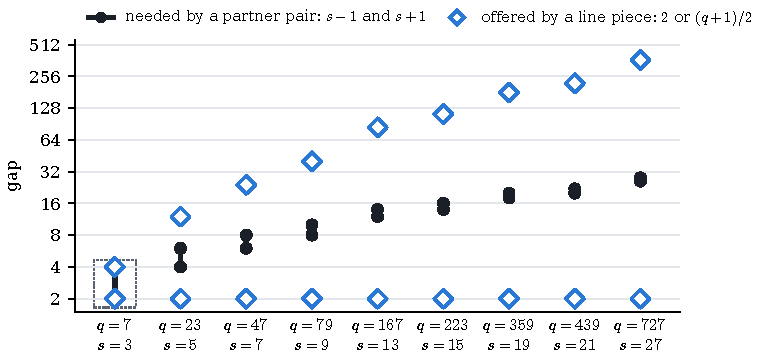
\includegraphics[width=0.78\textwidth]{sporadic_gaps.pdf}
\caption{Why standard line pieces work only for $q=7$.
In a line-piece regular member, each partner pair of fibres (Lemma~\ref{lem:slopes}) forces the intercept set $T$ of a line piece to be two-valued with gap $s-1$ or $s+1$ (black).
Standard line pieces offer only the gaps $2$ and $(q+1)/2$ (blue).
The two pairs agree only for $s=3$ (dashed box).
In every other member of Mathon's family, $s\pm1$ lies strictly between them.}
\label{fig:gaps}
\end{figure}

\begin{remark}\label{rem:twovalued}
The hypothesis on $T$ is used only to determine the possible gaps. For $q\in\{7,11,19,23,31\}$, an enumeration of all
$2^q$ subsets of $\F_q$ shows that the two-valued sets are exactly the translates of $\{0\}$, $N$, $\{0\}\cup Q$ and
$\F_q^\times$, with gaps $2$ and $\tfrac{q+1}2$; Conjecture~\ref{conj:twoval} asserts this for all $q$. Hence at
$q=23$ the conclusion of Theorem~\ref{thm:sporadic} holds for every $X$ that meets each fibre in a union of parallel
lines, whatever the intercepts. Proposition~\ref{prop:q23all} proves this independently for all template data.
\end{remark}

\subsection{Members fixed by \texorpdfstring{$h$}{h}}
Let $\omega$ generate $Q$, and let $h$ act by $(i,a,b)\mapsto(i,\omega a,\omega b)$ and fix $\infty$.
The blocks (M1) and (M2) are invariant under this scaling, so $h$ is an automorphism of $\Omega_q$ that fixes every fibre.
For $q=7$ it is the subgroup $C_3$ of $\Aut\OM$ that fixes every fibre, and the members it fixes are the centred ones.
Line pieces with $T$ a union of $\{0\},Q,N$ are $h$-invariant, but an $h$-invariant member need not be made of line pieces.

An $h$-invariant vector is constant on the $h$-orbits of a fibre (the origin and the half-lines through it), so a few
numbers per fibre describe it, and $Sx=\rho x$ becomes linear conditions on these numbers that couple only partner
fibres. An $h$-invariant function on a fibre is determined by two kinds of values.
One is its value $e_0$ at the origin.
The others are, for each slope $m$ with direction $d_m=(1,m)$ or $d_\infty=(0,1)$, its values $f_m^\pm$ on the two half-lines $\{td_m:\chi(t)=\pm1\}$.
Put $\alpha_m=(f_m^++f_m^-)/2$ and $\delta_m=(f_m^+-f_m^-)/2$, so that exactly one of them is $\pm1$ and the other is $0$, and put $A=\sum_m\alpha_m$.
Let $\sigma$ be the $(q+1)\times(q+1)$ matrix with $\sigma_{mm}=0$ and $\sigma_{mm'}=\chi(\ell_m(d_{m'}))$ for $m\ne m'$.
It satisfies $\sigma\sigma^\top=qI$ (a conference matrix in the general sense; it is neither symmetric nor skew), by the same character-sum identity $\chi*\chi=1-q\delta_0$ as Paley's matrices~\cite{Paley1933}.
Put $P=\sigma\delta$, i.e.\ $P_m=\sum_{m'\ne m}\sigma_{mm'}\delta_{m'}$.

\begin{proposition}\label{prop:hinv}
Let $x$ be the switching vector of an $h$-invariant member of $\Omega_q$, with $Sx=\eta qs\,x$ and $x_\infty=1$.
\begin{enumerate}
\item On fibre $i$ the sums of $x_i$ over the lines of slope $m$ depend only on whether the intercept is $0$, in $Q$ or in $N$:
\[
\Lambda_{i,m}(0)=e_0+(q-1)\alpha_m,\qquad \Lambda_{i,m}(Q)=A-\alpha_m+P_m,\qquad \Lambda_{i,m}(N)=A-\alpha_m-P_m,
\]
with $e_0,\alpha,P,A$ those of fibre $i$.
\item Put $u=\Lambda(0)-\Lambda(Q)$, $v=\Lambda(0)-\Lambda(N)$ and $w=\Lambda(Q)-\Lambda(N)=2P$. For every partner
pair $(i,m)$, $(j,m^*)$ with $m\in\mathcal M$,
\[
u_{j,m^*}=\Sigma_{ij}\,\frac{\eta s+1}2\,w_{i,m},\qquad v_{i,m}=-\Sigma_{ij}\,\frac{\eta s-1}2\,w_{j,m^*}.
\]
\item Consequently every fibre satisfies, for each slope $m$, the local conditions
\[
\begin{cases}
v_m\equiv0\pmod{s-\eta}\ \text{and}\ |P_m|\le 2q/(s+\eta), & m\in\mathcal M,\\
u_m\equiv0\pmod{s+\eta}\ \text{and}\ |P_m|\le 2q/(s-\eta), & m\in\mathcal P.
\end{cases}
\]
They involve only $q$, $s$ and $\eta$, not $i$ or $\Sigma$.
\end{enumerate}
\end{proposition}

\begin{proof}
(i) The line $\ell_m=0$ consists of the origin and the two half-lines of slope $m$.
A line $\ell_m=y$ with $y\ne0$ meets the line through the origin of slope $m'\ne m$ in the single point $td_{m'}$, where $t=y/\ell_m(d_{m'})$.
That point lies on the half-line of sign $\chi(y)\sigma_{mm'}$.
Summing $\alpha_{m'}+\chi(y)\sigma_{mm'}\delta_{m'}$ over $m'\ne m$ gives the formula.
(ii) By the remark after~\eqref{eq:slopes}, $q\,g_{i,m}=\Lambda_{i,m}-q\bar x_i$.
Write this mean-zero function as $a(\delta_0-1/q)+b\chi$.
Then $u=a-b$, $v=a+b$ and $w=2b$.
In the basis $(\delta_0-1/q,\chi)$, convolution with $\chi'$ acts by $(a,b)\mapsto(-a-qb,\ a-b)$, and convolution with $\tilde\chi'$ by $(a,b)\mapsto(-a+qb,\ -a-b)$; both follow from $\chi*\chi=1-q\delta_0$.
Comparing the $\chi$-coefficients in the two forms of (P) gives (ii).
(iii) By (ii), $u_{j,m^*}=\pm(s+\eta)P_{i,m}$ and $v_{i,m}=\pm(s-\eta)P_{j,m^*}$.
Moreover $|u|,|v|\le2q$, since every line sum lies in $[-q,q]$.
\end{proof}

At $q=7$ the line pieces of~\cite{Plummer442} satisfy (ii) with one side zero.
For example, fibres $1$ and $7$ of $\mathrm A_1$ (Remark~\ref{rem:q7}) have $(u,v,w)=(14,0,-14)$ and $(-14,-14,0)$, and $\Sigma_{17}=-1$ (Figure~\ref{fig:reduction}(a)).
A general $h$-invariant fibre mixes the states $\alpha$ and $\delta$ on different slopes, and (ii) couples it to $q+1$ other fibres.

\paragraph{The two-graph $\Omega_{23}$.} For $q=23$ we take the base $\Pal(25)$ and label $\F_{25}=\F_5[i]$, $i^2=2$,
by $\Z_{25}$ via $yi+z\mapsto5y+z$. The skew Latin square is the circulant one, $L(a,b)=b-a$ reduced to
$\pm1,\dots,\pm12$. Translating the labels by $5$ is the field translation by $i$. This is an automorphism of
$\Pal(25)$ that preserves $L$, and (M1), (M2) depend on the fibres only through $\Sigma$ and $L$, so it induces an
automorphism $t$ of $\Omega_{23}$ of order $5$.

\begin{proposition}\label{prop:q23h}
$\Omega_{23}$ has no regular member fixed by $h$: there is no $h$-invariant member that is an
$\srg(13226,6670,3363,3364)$ or an $\srg(13226,6555,3248,3249)$.
\end{proposition}
\begin{proof}
An $h$-invariant fibre is determined by its value at the origin and its values on the two half-lines of each slope,
which gives $2\cdot4^{q+1}$ states. By Proposition~\ref{prop:hinv}, we must choose one state per fibre so that (ii)
and (M) hold. Neither step below assumes that fibres are line pieces.

First, by meet-in-the-middle over the slopes, we list the \emph{local patterns}: the states that satisfy the local
conditions (iii), which are the same for every fibre. Second, we choose one local pattern per fibre by depth-first
search with forward checking. The constraints are the two equations of (ii) on each of the $p(q+1)/2$ partner pairs;
condition (M) is checked on complete assignments, and the symmetry $t$ is broken. Every solution is rebuilt as a vector
$x\in\{\pm1\}^{q^2p+1}$, and $Sx=\rho x$ is checked directly. Table~\ref{tab:search} gives the sizes. For $q=23$ there
is no solution for either sign of $\rho$.
\end{proof}

\begin{table}[h]
\centering\small
\begin{tabular}{rrrrrr}
\toprule
$q$ & $\rho$ & degree & local patterns & search nodes & solutions\\
\midrule
$7$ & $-21$ & $231$ & $6256$ & $418\,869$ & $15$\\
$7$ & $21$ & $210$ & $6256$ & $417\,337$ & $15$\\
$23$ & $-115$ & $6670$ & $206\,632$ & $284\,271\,840$ & $0$\\
$23$ & $115$ & $6555$ & $189\,142$ & $276\,655\,619$ & $0$\\
\bottomrule
\end{tabular}
\caption{The exact search for $h$-invariant members; at $q=23$ a fibre has $2\cdot4^{24}\approx5.6\cdot10^{14}$ states.}
\label{tab:search}
\end{table}

\begin{remark}[controls]\label{rem:search}
At $q=7$ the same search returns exactly the $15+15$ centred members, that is, the switching sets of the graphs
of~\cite{Plummer442} and their images under $\Aut\OM$. Requiring invariance under all of $\langle h,t\rangle$, with
$t\colon(i,u)\mapsto(i+3,u)$ of order $3$ (Section~\ref{sec:census}), leaves
exactly the graphs $\mathrm B_4,\dots,\mathrm B_9$ of~\cite[Table~1]{Plummer442}. At $q=23$ the two searches under
$\langle h\rangle$ took $47$ and $45$ CPU hours. Under $\langle h,t\rangle$, with $t$ the automorphism of order $5$ above, the search is much shorter: degree $6555$ is
excluded by (M) and the integrality of the fibre sums alone, and degree $6670$ after $63$ search nodes.
\end{remark}

\begin{figure}[t]
\centering
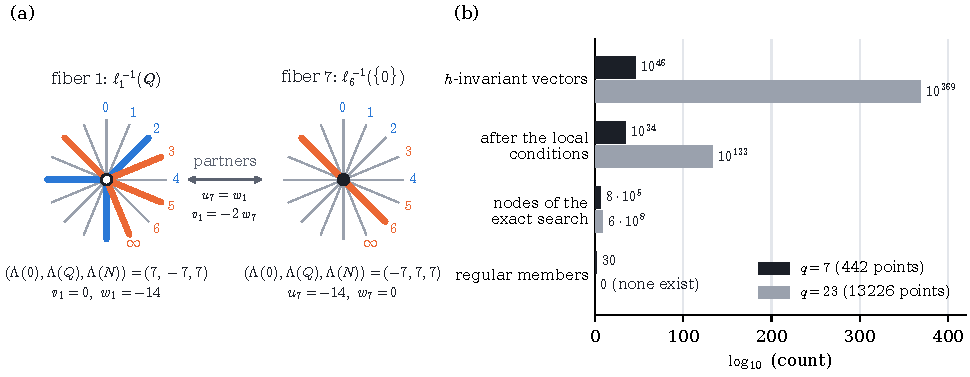
\includegraphics[width=\textwidth]{sporadic_reduction.pdf}
\caption{The local structure of $h$-invariant members, and the search it makes possible.
(a)~Two fibres of the graph $\mathrm A_1$ of~\cite{Plummer442} that are partners (Lemma~\ref{lem:slopes}), drawn by their $h$-orbits.
The dot is the origin, filled if it is switched.
Each diameter is the line through the origin of one slope, blue for $\mathcal M=\{0\}\cup Q$ and orange for $\mathcal P=N\cup\{\infty\}$.
Its half towards the label is $\{td_m:t\in Q\}$, and a half is drawn thick when it is switched.
Fibre $1$ is the line piece $\ell_1^{-1}(Q)$, which has the state $\delta$ on every slope except $1$.
Below each fibre are its line sums on the partner slopes $1$ and $6$, which satisfy the pair equations of Proposition~\ref{prop:hinv}(ii).
(b)~Sizes on a logarithmic scale for $q=7$ and $q=23$, both degrees together: all $h$-invariant switching vectors,
$(2\cdot4^{q+1})^p$ (out of $2^{441}$ and $2^{13225}$ in all); those whose fibres are all local patterns; search nodes
(for $q=23$ after breaking a symmetry of order $5$); and regular members found ($30$ centred members at $q=7$, none at
$q=23$).}
\label{fig:reduction}
\end{figure}
